\chapter{Neural Network Pruning}
\label{chap:neural_network_pruning}

\section{Introduction}
\label{sec:pruning_intro}

Within the framework established in Chapters ~\ref{chap:foundations} and ~\ref{chap:specialized_architectures}, pruning can be understood as a
constrained reduction of a trained network. The optimization perspective defines how
pruning error is measured, the architectural structure of the network determines which
components can be removed, and deployment metrics determine
whether pruning leads only to nominal sparsity or to practical savings.

Pruning is an established deep neural network compression technique. Its purpose is to remove non-critical active parameters or operations in a network in a way that preserves the overall behavior of the pruned network to be similar to a reference network. In this removal process, the actual topology of the network is modified by setting weights, channels, filters, layers, or other units to zero, by masking them, or by removing them completely. The mask decision is simultaneously a compression choice and an architectural one.

The relevance of pruning follows from the over-parameterised nature of modern
neural networks. Large models often contain substantial redundancy distributed
unevenly across layers and parameter groups \cite{denil2013predicting,michel2022not}. Table~\ref{tab:model_sizes}
illustrates the scale: each parameter requires 4 bytes at full precision (FP32)
or 2 bytes at half precision (FP16), placing a hard memory floor on deployment
before activations or caches are considered
\cite{He2016,devlin2019bert,radford2019language,touvron2023llama2,achiam2023gpt}.

\begin{table}[H]
	\centering
	\caption{Parameter counts and memory footprints for selected modern models.
		FP32 assumes 4 bytes per parameter; FP16 assumes 2 bytes per parameter.}
	\label{tab:model_sizes}
	\small
	\renewcommand{\arraystretch}{1.3}
	\begin{tabularx}{\textwidth}{lrrrX}
		\toprule
		\textbf{Model} & \textbf{Params} & \textbf{FP32 (GB)} & \textbf{FP16 (GB)}
		& \textbf{Notes} \\
		\midrule
		ResNet-50          & 25.6 M  & 0.10 & 0.05 & Image classification \\
		BERT-Base          & 110 M   & 0.44 & 0.22 & Encoder model \\
		GPT-2 (XL)        & 1.56 B  & 6.24 & 3.12 & Autoregressive model \\
		LLaMA-2 (7B)      & 6.74 B  & 26.9 & 13.5 & Large decoder model \\
		LLaMA-2 (70B)     & 68.9 B  & 275  & 138  & Requires multiple GPUs \\
		GPT-4             & --       & --   & --   & Parameters not publicly disclosed \\
		\bottomrule
	\end{tabularx}
\end{table}

A simple parameter count shows why sparsity cannot be interpreted as savings by itself. For example, a
70B-parameter model requires about 140\,GB in FP16 under dense storage, and setting half of
its weights to zero without any type of physical pruning does not change this footprint unless the representation or execution pattern
also changes. Prior work on sparse neural network execution shows that practical acceleration depends on whether the sparse pattern is exploitable by the software and hardware stack \cite{gale2020sparsegpu,cheng2024survey}.
The pruning problem is therefore not only to reduce a numerical count of weights, but to choose
which parameters or structures remain active under a given cost constraint. This leads us in the next section to
formalize this choice using mask variables~\cite{kwon2022fast}.



\section{Theoretical Framework of Pruning}
\label{sec:pruning_theoretical_framework}
Pruning can be formalized as a constrained optimization problem where the goal is to find a binary mask that selects which parameters to keep while minimizing the loss increase. The mask effectively defines the pruned network by zeroing out the parameters that are removed. The optimization problem can be expressed in both constrained and regularized forms, and its solution is generally NP-hard ~\cite{dong2017learning}, leading to the use of approximate criteria based on Taylor expansions of the loss function.

\subsection{Formal Problem Formulation}
\label{subsec:pruning_formal_problem}

Given a parameterized network $f(\cdot;\Theta)$ whose $P$ parameters are
stored in $\Theta \in \mathbb{R}^P$, a binary mask $M \in \{0,1\}^P$ is
chosen such that those parameters selected to be kept (whose mask value is
$1$) can be retrieved and those not (mask value $0$) excluded from further
calculation by computing $f(x; M \odot \Theta)$, which zeros out parameters
for which $M_i = 0$ by elementwise product.

The goal is then to find the mask $M$ and the remaining weights $\Theta$ that
keep the loss $\mathcal{L}$ as low as possible while meeting a budget on how
many parameters are retained:
\begin{equation}
	\min_{\Theta, M}\; \mathcal{L}(M \odot \Theta)
	\quad
	\text{subject to}
	\quad
	\frac{\lVert M \rVert_0}{P} \le \kappa,
	\label{eq:constrained}
\end{equation}
where $\lVert M \rVert_0$ counts the nonzero entries of $M$ and $\kappa \in
(0,1]$ is the target density. In practice this hard constraint is often
replaced by a regularised objective that avoids having to fix $\kappa$ in
advance:
\begin{equation}
	\min_{\Theta, M}\; \mathcal{L}(M \odot \Theta) + \lambda\,\Omega(M),
	\label{eq:regularised}
\end{equation}
where $\lambda$ controls how aggressively compression is penalised and
$\Omega(M)$ can capture parameter count, memory footprint, or latency
depending on the deployment target. This regularised form folds the budget into the objective instead of enforcing it as a hard constraint (Eq.~\eqref{eq:regularised}).

Finding an optimal pruning solution is generally NP-hard, since the search
space grows exponentially with the number of parameters~\cite{dong2017learning}.
Practical methods thus resort to approximate measures which evaluate how pruning a parameter or structure affects performance without considering all possible masks. Such measures can be obtained by approximating the change in training loss due to pruning, commonly through a Taylor expansion \cite{molchanov2017variational}.

\subsection{Taylor Expansion Analysis of Pruning Loss}
\label{subsec:taylor_pruning_loss}

The impact of pruning on the loss can be characterised by expanding the loss around the trained weights $\Theta^*$. Let $\delta\Theta = M \odot \Theta^* - \Theta^*$ be the perturbation induced by masking:

\begin{equation}
	\Delta\mathcal{L}
	\approx
	\underbrace{\nabla\mathcal{L}(\Theta^*)^\top \delta\Theta}_{\text{1st order}}
	+
	\frac{1}{2}\,\underbrace{\delta\Theta^\top H(\Theta^*)\,\delta\Theta}_{\text{2nd order}}
	+ \mathcal{O}(\norm{\delta\Theta}^3),
	\label{eq:taylor}
\end{equation}

where $H(\Theta^*) \in \R^{P \times P}$ is the Hessian of the loss at $\Theta^*$. The expansion separates the pruning effect into first-order sensitivity and second-order curvature (Eq.~\eqref{eq:taylor}). The first-order term measures how sensitive the loss is to the direction of weight removal: a weight with a large gradient, when removed, shifts the loss proportionally. What the second-order term adds is curvature. It captures how steeply the gradient itself changes as weights are zeroed out, which determines whether removing a small weight from a sharp loss valley is actually safe. At a stationary point of training where $\nabla\mathcal{L}(\Theta^*) \approx 0$, the first-order term vanishes and curvature becomes the decisive quantity.

Depending on which terms are retained and how $H$ is approximated, this expansion gives rise to the full family of saliency criteria used in practice, from magnitude scoring (zeroth order, which ignores both terms and uses weight magnitude as a proxy) through gradient-based methods (first order) to blockwise curvature methods, each of which is developed in Section~\ref{sec:pruning_criteria} and applied to specific methods in Chapters ~\ref{chap:related_work_pruning_structured} and~\ref{chap:related_work_pruning_unstructured}.

For second-order criteria, the same Taylor expansion can be used while keeping
the curvature term. This gives a more accurate estimate of the loss change,
but it also requires approximating the Hessian, which is expensive at modern
scales. The original OBD criterion is a simple diagonal approximation, while
later methods apply the same idea blockwise to recover tractability.

\subsection{Optimal Brain Damage and Optimal Brain Surgeon}
\label{subsec:obd_obs}

OBD \cite{lecun1989optimal} is the simplest instantiation of the second-order
term of the Taylor expansion: it assumes the Hessian is diagonal and applies no compensating correction to the remaining weights after the removal of a single weight,
so the saliency of each weight reduces to

\begin{equation}
	S_i^{\mathrm{OBD}} = \frac{1}{2}\, H_{ii}\,\theta_i^2.
	\label{eq:obd}
\end{equation}

Under the OBD approximation, saliency becomes a Hessian-weighted square of the parameter (Eq.~\eqref{eq:obd}). This makes ranking cheap, but it ignores interactions between
weights. OBS \cite{hassibi1993second} drops the diagonal assumption
entirely: after each removal it solves for the optimal correction of the remaining weights
induced by removing a weight, achieving strictly lower loss increase than OBD. The price is the full
inverse Hessian, which is intractable at modern scales. This is where the
connection to modern post-training compression becomes direct: later methods recover
tractability by applying OBS-style updates blockwise, one layer at a time,
with the resulting per-layer formula derived in Section~\ref{subsec:second_order_criteria}
\cite{frantar2023sparsegpt,frantar2022gptq}.

\subsection{Density, Sparsity, and Effective Topology}
\label{subsec:density_sparsity_topology}

The saliency criteria above produce a score for each weight, but before
deciding which weights to remove it is useful to establish what a removal
decision actually means quantitatively. Given $N_\mathrm{act}$ active
(nonzero) parameters out of a total of $P$, the \emph{density} and
\emph{sparsity} of the pruned network are
\begin{equation}
	\rho = \frac{N_\mathrm{act}}{P}, \qquad s = 1 - \rho.
	\label{eq:density_sparsity}
\end{equation}

Density and sparsity define how many parameters remain active (Eq.~\eqref{eq:density_sparsity}). They say nothing about where the removed weights were located.
The same sparsity $s = 0.90$ can describe a network where zeros are scattered
uniformly across all layers, leaving every operation dense but smaller, or
one where zeros are concentrated in a few layers, leaving those layers nearly
intact while others are almost entirely zeroed out, or one where the pattern is
irregular enough that hardware cannot skip the zeroed operations without
specialised sparse-format support \cite{hoefler2021sparsity}. A sparsity ratio
is therefore a necessary but insufficient description of a pruned network; what
matters equally is the \emph{structure} of the removal pattern. This is what
the next section formalises.


%% ----------------------------------------------------------------------------
\section{Pruning Structures}
\label{sec:pruning_structures}
%% ----------------------------------------------------------------------------

The pattern in which weights are removed determines whether the resulting
model can be accelerated on real hardware, and how much freedom the pruning
criterion has in choosing which units to remove
\cite{cheng2024survey,hoefler2021sparsity}. Three structural regimes cover
the main options, each sitting at a different point on the trade-off between
pruning flexibility and deployment efficiency.

\subsection{Unstructured Pruning}
\label{subsec:unstructured_pruning}

\keyterm{Unstructured pruning} removes individual scalar weights without any
constraint on their positions in the weight matrix \cite{han2015deep}.
Formally, given an importance score $S(\theta_i)$ for each parameter
$\theta_i$, the binary mask $M \in \{0,1\}^P$ retains the top-$\kappa$
fraction of weights by score:
\begin{equation}
	M_i = \mathbf{1}\!\left[S(\theta_i) \ge \tau_\kappa\right],
	\label{eq:unstructured_mask}
\end{equation}
where $\tau_\kappa$ is the $(1-\kappa)$ quantile of the score distribution.
This connects the density constraint to a concrete mask rule: keep the weights above the score threshold and zero out the rest (Eqs.~\eqref{eq:constrained} and~\eqref{eq:unstructured_mask}).

This regime offers the most freedom because each weight is scored
independently, which tends to produce the best accuracy at a given sparsity
level \cite{frankle2018lottery}. The cost is deployment: the resulting zero
pattern is irregular, and standard hardware cannot skip zeroed multiplications
without sparse storage formats, such as compressed sparse row (CSR) formats that store only nonzero values and their indices, and specialised kernels that skip zero-valued operations. In practice, latency
reductions are modest unless sparsity exceeds roughly 90\%, and even then only
when paired with sparse execution support \cite{gale2020sparsegpu}.

\subsection{Semi-Structured Pruning ($N\!:\!M$ Sparsity)}
\label{subsec:semi_structured_pruning}

\keyterm{$N\!:\!M$ sparsity} is a constrained form of unstructured pruning
that imposes a regular local pattern \cite{mishra2021accelerating}. Instead
of allowing arbitrary weights to be removed anywhere in the matrix, the weight
vector is partitioned into consecutive non-overlapping groups $\mathcal{G}$ of
$M$ elements. Within each group, exactly $N$ elements are retained and the
remaining $M-N$ are zeroed:
\begin{equation}
	\lVert m_\mathcal{G} \rVert_0 = N \qquad \forall\,\mathcal{G},\;|\mathcal{G}|=M,
	\label{eq:nm_constraint}
\end{equation}
Here $m_\mathcal{G} \in \{0,1\}^M$ is the mask restricted to group
$\mathcal{G}$ and $\lVert \cdot \rVert_0$ counts its nonzero entries. The
constraint forces each local group to keep the same number of weights, which
makes the sparsity pattern more predictable than unconstrained unstructured
pruning.

A widely used instance of semi-structured sparsity is the 2:4 pattern,
where only two weights are kept in every group of four weights
\cite{pytorch2024semistructured,hu2024accelerating}. This gives the
hardware a predictable sparse layout based on small weight groups. NVIDIA
Ampere Sparse Tensor Cores support this fine-grained sparsity pattern and can
exploit it for faster matrix multiplication when the required 2:4 constraint
is satisfied \cite{nvidia2020a100,mishra2021accelerating}.

After arbitrary weight removal and local group-wise constraints, a question
that may come to mind is what happens if we try to remove coarser
structures, such as complete architectural components. This is the topic of
the next point.

\subsection{Structured Pruning}
\label{subsec:structured_pruning}

\keyterm{Structured pruning} removes entire vectors or submodules rather than
individual weights, producing a strictly smaller dense model with no irregular
sparsity \cite{li2017pruning}. Because the result is a standard dense matrix,
no sparse storage format or specialised kernel is needed; the compressed model
runs on any hardware that supports ordinary matrix multiplication.

The removable unit depends on the architecture. In a convolutional network it is typically a filter or a channel; in a fully connected network it may be a neuron or a hidden dimension. The specific Transformer instantiation is covered later in Section~\ref{sec:pruning_transformers}.

Formally, removing rows and columns from a weight matrix $W \in \R^{m \times n}$
using a row mask $r \in \{0,1\}^m$ and a column mask $c \in \{0,1\}^n$ yields
the submatrix
\begin{equation}
	W' = W[\mathcal{R}, \mathcal{C}] \in \R^{m' \times n'},
	\label{eq:structured_submatrix}
\end{equation}
where $\mathcal{R} = \{i : r_i = 1\}$ and $\mathcal{C} = \{j : c_j = 1\}$
are the index sets of retained rows and columns, and $m' = |\mathcal{R}|$,
$n' = |\mathcal{C}|$ are the reduced dimensions. The point of this construction is that structured pruning produces a smaller dense matrix, not a dense matrix with scattered zeros (Eq.~\eqref{eq:structured_submatrix}).

Figure~\ref{fig:structures} illustrates how the three regimes differ in their
removal patterns. In the unstructured case, zeroed weights are scattered
arbitrarily across the matrix, giving maximum freedom but producing no
contiguous blocks that hardware can skip. Semi-structured sparsity resolves
this by imposing a fixed retention ratio within each local group, aligning
the pattern with dedicated hardware engines. Structured pruning goes further:
removing entire rows or columns leaves a fully dense submatrix with no
irregular zeros and no sparse-format overhead.


\begin{figure}[H]
	\centering
	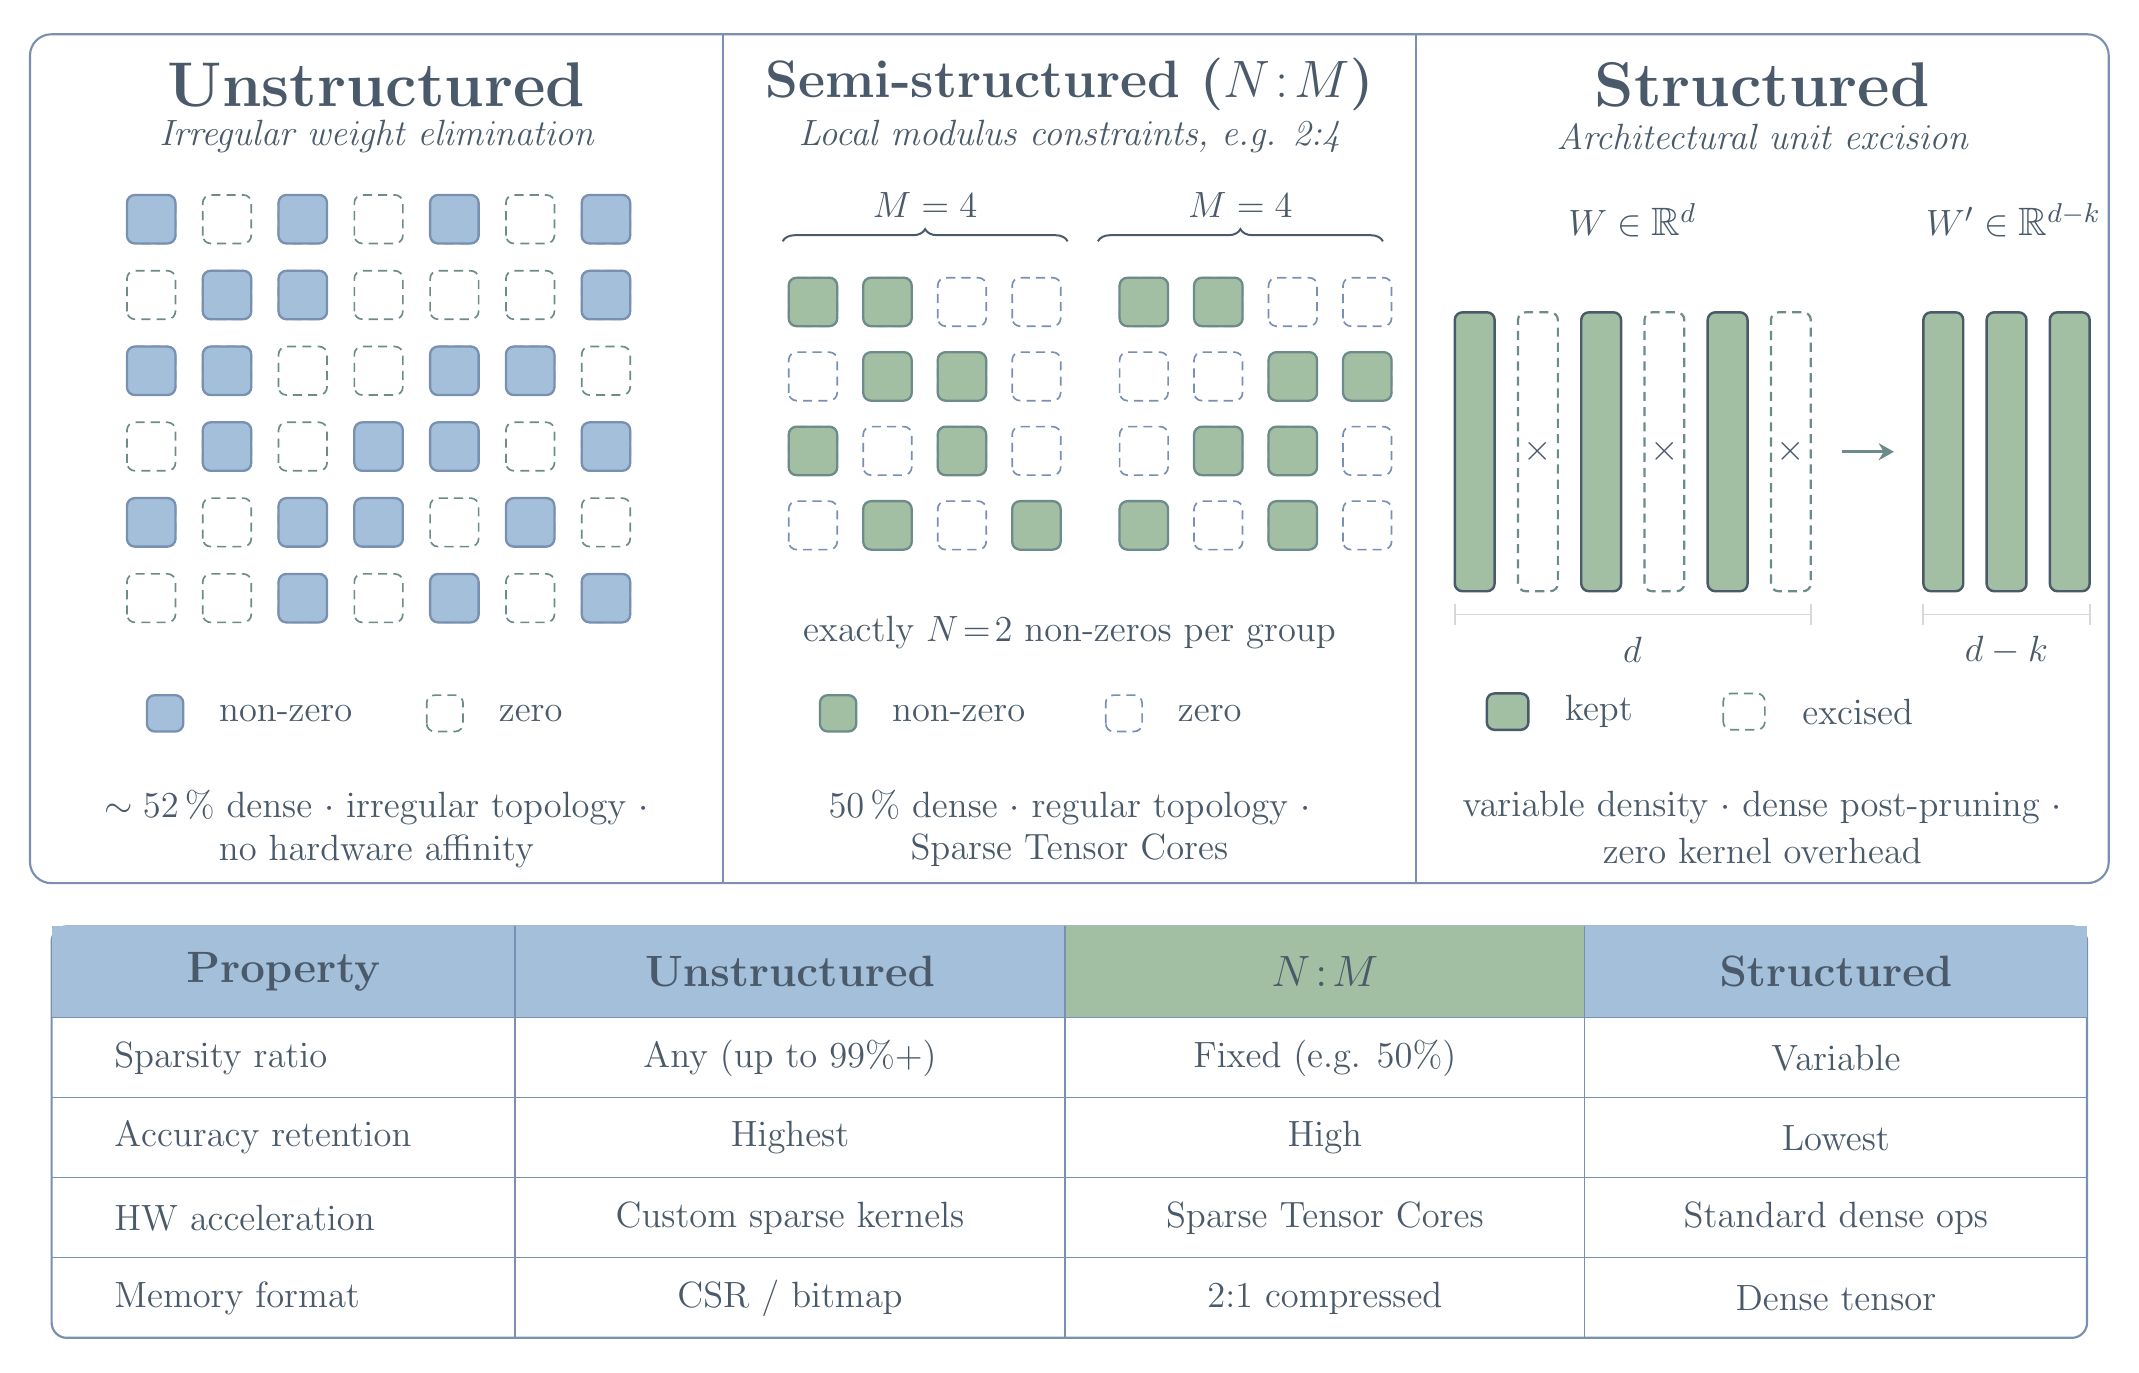
\includegraphics[width=\textwidth]{figures/compression/pruning_s_ss_ns.PNG}
	\caption{Comparison of unstructured, semi-structured, and structured sparsity
		patterns in a weight matrix.
%	White cells indicate removed weights. Unstructured
%		sparsity scatters zeros freely across the matrix; semi-structured sparsity
%		enforces a fixed retention ratio within each local group; structured sparsity
%		removes entire rows or columns, yielding a dense submatrix.
	}
	\label{fig:structures}
\end{figure}

%% ----------------------------------------------------------------------------
\section{Pruning Criteria}
\label{sec:pruning_criteria}

While the sparsity structure determines the shape and hardware footprint of the
compressed model, it says nothing about \emph{which} specific weights or units
should be removed. That decision is governed by the pruning criterion: given a
fixed removal budget, the criterion ranks the parameters or structures by their
estimated importance to the network's output, so that the least important ones
are removed first.
%% ----------------------------------------------------------------------------

A \keyterm{pruning criterion} assigns an importance score $S(\theta_i)$ (or
$S(g)$ for a structured group $g$) that serves as a proxy for the loss change
$\Delta\mathcal{L}$ induced by removing that element.  The ideal criterion
ranks units by \emph{true irreplaceability}: the unit with the lowest true
loss impact should be removed first.

\subsection{Magnitude-Based Criteria}
\label{subsec:magnitude_based_criteria}

The most common zeroth-order criterion evaluates a weight by its absolute value \cite{han2015learning}:
\begin{equation}
	S_{\mathrm{mag}}(w_i) = |w_i|.
	\label{eq:mag}
\end{equation}
For structured groups (e.g.\ a convolutional filter
$W_g \in \R^{c_\mathrm{out} \times c_\mathrm{in} \times k \times k}$), the
same idea is applied to the whole group rather than to one scalar weight. Common choices are the $\ell_1$, $\ell_2$, and $\ell_\infty$ norms:
\begin{align}
	S_g^{(1)} &= \norm{W_g}_1 = \sum_{i} |w_{g,i}|, \label{eq:mag_l1} \\
	S_g^{(2)} &= \norm{W_g}_2 = \sqrt{\sum_{i} w_{g,i}^2}, \label{eq:mag_l2} \\
	S_g^{(\infty)} &= \norm{W_g}_\infty = \max_i |w_{g,i}|. \label{eq:mag_linf}
\end{align}
These group scores extend the scalar magnitude rule to structured units: first score a whole tensor, then remove the groups with the smallest values. The $\ell_1$ score measures total absolute magnitude, the $\ell_2$ score measures Euclidean energy, and the $\ell_\infty$ score keeps only the largest entry in the group (Eqs.~\eqref{eq:mag}, \eqref{eq:mag_l1}, \eqref{eq:mag_l2}, and~\eqref{eq:mag_linf}).

The $\ell_2$ norm is the most common because it is differentiable and
rotation-invariant.  The $\ell_\infty$ norm is sensitive to outliers and
is less often used alone.

\textbf{Interpretation.} At a stationary point with a well-conditioned
Hessian, $S_{\mathrm{2nd}} = \tfrac{1}{2} H_{ii} w_i^2 \propto w_i^2$ if
$H_{ii}$ is approximately constant across parameters.  Under this assumption,
ranking by $|w_i|$ is equivalent to ranking by the second-order saliency \cite{lecun1989optimal}.
When Hessian diagonal entries vary greatly across layers (which they do in
practice), magnitude alone may rank units from poorly-conditioned layers too
aggressively.

\subsection{Gradient-Based Criteria}
\label{subsec:gradient_based_criteria}

First-order saliency estimates include the effect of the local gradient \cite{molchanov2017variational}:
\begin{equation}
	S_{\mathrm{grad}}(w_i)
	= \left|\frac{\partial\mathcal{L}}{\partial w_i}\cdot w_i\right|.
	\label{eq:grad}
\end{equation}
This is obtained from the first-order Taylor term with $\delta w_i = -w_i$
(complete removal), which turns the local gradient into a gradient-weight saliency score (Eq.~\eqref{eq:grad}). For structured pruning, the same criterion can be
extended to a removable group by summing over all constituent parameters:
\begin{equation}
	S_{\mathrm{grad}}(g)
	= \left|\sum_{i \in g}\frac{\partial\mathcal{L}}{\partial w_i}\cdot w_i\right|.
	\label{eq:grad_group}
\end{equation}
This produces one importance value for the whole group, not one value per scalar weight (Eq.~\eqref{eq:grad_group}) \cite{molchanov2017variational}.

\subsection{Second-Order Criteria}
\label{subsec:second_order_criteria}
For second-order criteria, the Taylor expansion is kept to the curvature term, which gives a more accurate estimate of the loss change but requires approximating the Hessian. The original OBD criterion is a simple diagonal approximation, while later methods apply the same idea blockwise to recover tractability.
There are two main approaches to second-order criteria: the diagonal approximation of OBD and the blockwise inverse Hessian of OBS.

\paragraph{Diagonal approximation (OBD style).}
\begin{equation}
	S_{\mathrm{2nd}}(w_i) = \frac{1}{2}\,H_{ii}\,w_i^2.
	\label{eq:second_order}
\end{equation}
The diagonal curvature term used in this score can be estimated from the Gauss-Newton approximation to the Hessian,
which requires computing per-sample gradients:
\begin{equation}
	H \approx G^\top G, \qquad G_{ij} = \frac{\partial \ell_j}{\partial w_i},
\end{equation}
where $\ell_j$ is the loss on sample $j$. The diagonal is then
$H_{ii} \approx \sum_j G_{ij}^2$, giving the curvature factor used by the second-order score (Eq.~\eqref{eq:second_order}).

\paragraph{Blockwise inverse Hessian.}
The full OBS correction is too expensive to apply to all parameters at once, so modern methods apply the same idea locally inside large linear layers \cite{hassibi1993second,frantar2023sparsegpt}. In a layer with weight matrix $W \in \R^{m \times n}$, the calibration activations are collected in $X \in \R^{n \times N}$, with one column per calibration sample. These activations give the empirical input Hessian $\hat{H}=XX^\top/N$, which describes how input directions interact inside the layer. The layer is then processed column by column: when one weight is removed, the remaining weights in the current block are adjusted so that the layer output changes as little as possible.
\begin{equation}
	W_{:,j}' = W_{:,j} - \frac{w_{:,j}}{[\hat{H}^{-1}]_{jj}}\, w_{:,j}^\top \hat{H}^{-1}_{j+1:, j},
	\label{eq:sparsegpt}
\end{equation}
This correction, written in Eq.~\eqref{eq:sparsegpt}, carries the pruning error into the surviving columns instead of leaving it concentrated at the removed weight. After each removal, the remaining inverse Hessian is updated efficiently, so the next pruning decision is made with the current block state rather than the original dense one. The total cost is $O(n^3 + mn^2)$ per layer.

\subsection{Activation-Aware Criteria}
\label{subsec:activation_aware_criteria}

Some criteria scale saliency by the activation statistics at the weight's
input. Concretely, the weight magnitude is multiplied by the $\ell_2$ norm of
the input feature it processes \cite{sun2023simple}:
\begin{equation}
	S_{\mathrm{act}}(W_{i,j}) = |W_{i,j}|\cdot\norm{x_j}_2,
	\label{eq:wanda}
\end{equation}
where $\norm{x_j}_2$ is the $\ell_2$ norm of the $j$-th input feature
computed over a calibration set of $N$ samples calculated as shown in Eq.~\eqref{eq:rms_activation}:
\begin{equation}
	\label{eq:rms_activation}
	\norm{x_j}_2 = \sqrt{\sum_{s=1}^{N} x_{s,j}^2\,}.
\end{equation}
This equals $\sqrt{N}$ times the root-mean-square (RMS) of that feature's
activations. RMS measures how much energy a feature carries on average
across inputs. A feature with consistently large activations has high RMS.
One that is rarely triggered has low RMS and contributes little to the
output regardless of its associated weight's magnitude. Equation~\eqref{eq:wanda}
makes the criterion sensitive to both: a small weight on a high-RMS feature
scores higher than a larger weight on a near-silent one.

Activation magnitudes are distributed unevenly across input features
\cite{sun2023simple,wei2022outlier}. Magnitude-only scoring ignores this.
It assigns identical importance to a weight on a high-energy feature and to
an equally large weight on a near-zero feature, systematically
underestimating the contribution of the first group. Scaling by
$\norm{x_j}_2$ corrects that bias directly.

\subsection{Learnable and Adaptive Criteria}
\label{subsec:learnable_adaptive_criteria}

A fourth family introduces \emph{trainable mask scores} $v \in \R^P$ that are optimised jointly with weights \cite{louizos2018learning,mallya2018packnet}:
\begin{equation}
	M_i = \sigma\!\left(\frac{v_i - \bar{v}}{\epsilon}\right),
	\quad
	\text{or}
	\quad
	M_i = \mathbf{1}[v_i \ge \tau],
	\label{eq:learnable}
\end{equation}
The mask can be kept soft during training or converted into a hard keep/remove decision (Eq.~\eqref{eq:learnable}). The discrete threshold is approximated during backpropagation by a straight-through estimator \cite{bengio2013estimating}, which passes the gradient through the threshold as if it were the identity. The learning objective then adds a sparsity penalty so that accurate but dense masks are discouraged:
\begin{equation}
	\mathcal{L}_{\mathrm{sparse}} = \mathcal{L}(\Theta, M(v)) + \lambda \norm{v}_1.
	\label{eq:learnable_loss}
\end{equation}
This objective balances task performance against mask sparsity (Eq.~\eqref{eq:learnable_loss}).

These approaches are valuable especially in the setting where the training
distribution is accessible and the budget for mask optimisation is not the
constraint. At moderate sparsities in fine-tuning, they outperform static
criteria \cite{sanh2020movement,louizos2018learning}.

\subsection{Criterion Comparison}
\label{subsec:criterion_comparison}

Table~\ref{tab:criterion_comparison} places the criteria of this section side by
side. Read from top to bottom, it traces a single trade-off: the cheaper
criteria near the top observe only the weights themselves, while the richer ones
below require gradients, curvature, activations, or a training signal. That extra
information is precisely what buys the accuracy gains in the last column. The
table is therefore best read as a map from \emph{what a criterion is allowed to
observe} to \emph{how well it ranks units for removal}, which is the trade-off a
practitioner balances against the available data and compute budget.

\begin{table}[H]
	\centering
	\caption{Summary comparison of pruning criteria.}
	\label{tab:criterion_comparison}
	\renewcommand{\arraystretch}{1.5}
	\begin{tabularx}{\textwidth}{lXXccl}
		\toprule
		\textbf{Criterion} & \textbf{Information used}
		& \textbf{Data needed}
		& \textbf{Grad?} & \textbf{$H$?}
		& \textbf{Typical accuracy} \\
		\midrule
		Magnitude & Weight values only
		& None & No & No & Baseline \\
		Gradient (Taylor) & Gradient $\times$ weight
		& Train/calib & Yes & No & +1--3\% over mag \\
		OBD (\S\ref{subsec:obd_obs}) & Diag.\ curvature
		& Train/calib & Yes & Diag & +1--5\% over mag \\
		Blockwise OBS (\S\ref{subsec:second_order_criteria}) & Full curvature per layer
		& Calibration & No & Block & Best (post-train) \\
		Activation-weighted & Magnitude $\times$ activation
		& Calibration & No & No & Strong post-train \\
		Learned / trajectory mask & Score trajectory
		& Fine-tune & Yes & No & Best for fine-tune \\
		\bottomrule
	\end{tabularx}
\end{table}

%% ----------------------------------------------------------------------------
\section{Pruning Strategies}
\label{sec:pruning_strategies}
%% ----------------------------------------------------------------------------

The criteria defined above state \emph{what} to remove. A related question is
\emph{when} this removal occurs and when to let the model recover in between
removals. A pruning schedule describes the pattern of mask updates and
recoveries during the course of training or preparing for inference, which is
what this section covers.

\subsection{One-Shot Pruning}
\label{subsec:one_shot_pruning}

In \keyterm{one-shot pruning}, importance scores are computed once from the
fully trained model and all removal decisions are made in a single pass
\cite{han2015deep}. Algorithm~\ref{alg:one_shot} shows the procedure.

\begin{algorithm}[H]
	\SetAlgoLined
	\KwIn{Trained model $f(\cdot;\Theta)$, target density $\kappa$}
	\KwOut{Pruned model $f(\cdot; M \odot \Theta)$}
	Compute $S(\theta_i)$ for all $i \in [P]$\;
	Set threshold $\tau \leftarrow$ $(1-\kappa)$ quantile of $\{S(\theta_i)\}$\;
	$M_i \leftarrow \mathbf{1}[S(\theta_i) \ge \tau]$\;
	\textbf{Optional:} fine-tune $\Theta$ with $M$ fixed\;
	\Return $M \odot \Theta$\;
	\caption{One-Shot Pruning}
	\label{alg:one_shot}
\end{algorithm}

One-shot pruning requires no additional training rounds and can be applied
directly to a pretrained model, which makes it simple to run. But that
simplicity has a cost. All removal decisions come from a single pass over the
loss landscape on a small calibration set, with no opportunity for the model
to recover between mask updates. Accuracy at a given sparsity is lower than
for iterative methods \cite{han2015deep,zhu2018prune}.

\subsection{Iterative Pruning and Recovery}
\label{subsec:iterative_pruning}

\keyterm{Iterative pruning} directly addresses the limitation of one-shot
pruning by interleaving mask updates with weight recovery steps \cite{zhu2018prune}. Instead of removing
all targeted weights at once, the model is pruned gradually over $R$ rounds,
with a fine-tuning phase after each round to let the remaining weights
compensate for what was removed. Algorithm~\ref{alg:iterative} shows a
common formulation using a cubic sparsity schedule.

\begin{algorithm}[H]
	\SetAlgoLined
	\KwIn{Trained model $\Theta$, target density $\kappa$, rounds $R$}
	\KwOut{Pruned model $M \odot \Theta$}
	$\kappa_0 \leftarrow 1.0$ \tcp*{start fully dense}
	\For{$r = 1$ \KwTo $R$}{
		$\kappa_r \leftarrow \textsc{Schedule}(\kappa,\, r,\, R)$ \tcp*{interpolate density toward target}
		Compute scores $S(\theta_i)$ on current $\Theta$ \tcp*{re-evaluate importance}
		Update mask $M$ to density $\kappa_r$ \tcp*{remove lowest-scoring units}
		Fine-tune $\Theta$ with $M$ fixed for $T_r$ steps \tcp*{recover accuracy}
	}
	\Return $M \odot \Theta$\;
	\caption{Iterative Pruning}
	\label{alg:iterative}
\end{algorithm}

The $\textsc{Schedule}$ function can take many forms such as linear, cubic,
cosine, or step, and the choice is often borrowed directly from learning
rate scheduling practice, since both problems share the same goal of
controlling how aggressively a quantity changes over the course of training
\cite{zhu2018prune}. Figure~\ref{fig:schedules} illustrates several common
variants.

\begin{figure}[H]
	\centering
	\begin{tikzpicture}
		\begin{axis}[
			width=0.92\linewidth, height=5.5cm,
			xlabel={Round ($r/R$)},
			ylabel={Sparsity $s_r$ (\%)},
			xmin=0, xmax=1, ymin=0, ymax=95,
			legend pos=south east,
			legend style={font=\small},
			grid=both, grid style={gray!15},
			xtick={0,0.25,0.5,0.75,1.0},
			ytick={0,20,40,60,80,90},
			title={Sparsity Schedules for Iterative Pruning ($\kappa = 0.10$)},
			title style={font=\small\bfseries},
			]
			\addplot[very thick, colBlueBorder, domain=0:1, samples=50]
			{90 * x};
			\addlegendentry{Linear}
			\addplot[very thick, headergreen, domain=0:1, samples=50]
			{90 * (1 - (1-x)^3)};
			\addlegendentry{Cubic (front-loaded)}
			\addplot[very thick, actreddark, const plot]
			coordinates {(0,0)(0.2,30)(0.4,60)(0.6,75)(0.8,85)(0.9,90)(1,90)};
			\addlegendentry{Step}
			\addplot[very thick, slateblue, domain=0:1, samples=50]
			{90 * 0.5 * (1 - cos(deg(pi * x)))};
			\addlegendentry{Cosine}
		\end{axis}
	\end{tikzpicture}
	\caption{ Variants of sparsity schedules}
%		Sparsity schedules for iterative pruning targeting 90\% sparsity
%		over $R$ rounds. Cubic and cosine schedules slow down near the target,
%		giving the model time to stabilise before the final mask is frozen;
%		linear and step schedules do not.}
	\label{fig:schedules}
\end{figure}

Linear growth applies equal increments each round, so the removal rate at
the end of training is the same as at the start, with no settling period at
high sparsity.
Cubic growth concentrates most of the pruning early: by $r/R = 0.5$ roughly
87\% of the target sparsity budget is already spent, and the remaining rounds
operate at near-final density with small incremental changes.
Step schedules skip continuous interpolation and instead apply discrete jumps
at fixed intervals, holding the mask constant between updates.
Cosine growth starts slowly and accelerates toward the midpoint, then
decelerates as sparsity approaches the target.
The last rounds under cosine resemble those of cubic. Both avoid committing
large removals at high sparsity, where each pruned weight carries a larger
marginal effect on the loss \cite{zhu2018prune}.

\subsection{Pruning During Training}
\label{subsec:pruning_during_training}

A third family integrates sparsity directly into the optimisation loop by
adding a regularisation term to the training loss, typically an $\ell_1$
penalty of the form $\lambda \sum_i |\theta_i|$ \cite{liu2017learning}.
This encourages weights toward zero throughout training, so that sparsity
emerges gradually rather than being imposed after the fact \cite{han2015deep,guo2016dynamic}. Weights that fall
below a threshold are later hard-pruned. The main requirement is access to
the full training distribution, which makes this approach most suitable when
training from scratch or during a supervised fine-tuning stage, rather than
for post-hoc compression of a frozen model.

\subsection{Post-Training Pruning}
\label{sec:post_training_pruning}

\keyterm{Post-training pruning} applies pruning to a frozen pretrained model
using only a small calibration set, without any gradient updates to the
original training loss \cite{frantar2023sparsegpt}. This makes it the
practical default for large pretrained networks, where full retraining over
the original training distribution is prohibitively expensive.

The procedure runs in four steps. First, a small calibration set of a few
hundred samples is forwarded through the frozen model to collect
layer-wise input activation statistics. Second, those statistics are combined
with the weight values to compute a saliency score $S(\theta_i)$ for each
weight or group. Third, the lowest-scoring units are zeroed out to produce
the binary mask $M^*$. Fourth, an optional weight correction step adjusts
the values of the remaining weights in each layer to compensate for the
damage caused by the removals, an idea inherited from OBS and applied
blockwise in modern post-training methods \cite{frantar2023sparsegpt}.
Figure~\ref{fig:ptp_pipeline} summarises these steps.

\begin{figure}[H]
	\centering
	\begin{adjustbox}{max width=\linewidth}
	\begin{tikzpicture}[
		font=\small,
		box/.style={rectangle, rounded corners=3pt, draw=colBlueBorder, fill=colBlue!15,
			minimum width=2.8cm, minimum height=0.7cm, align=center},
		data/.style={rectangle, rounded corners=3pt, draw=headergreen, fill=colGreen!25,
			minimum width=2.8cm, minimum height=0.7cm, align=center},
		arr/.style={-Stealth, thick, colBlueBorder}
		]
		\node[data]  (pretrain)   {Pretrained\\model $\Theta^*$};
		\node[data, below=0.5cm of pretrain] (calib)
		{Calibration\\set ($\le$512 samples)};
		\node[box, right=1.2cm of calib]  (stats)
		{Collect input\\activations\\per layer};
		\node[box, right=0.8cm of stats]  (score)
		{Compute saliency\\score $S(\theta_i)$\\per weight/group};
		\node[box, right=0.8cm of score]  (mask)
		{Zero out\\lowest-scoring\\units: mask $M^*$};
		\node[box, right=0.8cm of mask]   (opt)
		{Correct remaining\\weights to offset\\removed units};
		\node[data, below=0.7cm of opt]   (pruned)
		{Pruned model\\$M^* \odot \Theta^*$};

		\draw[arr] (pretrain) -| (stats);
		\draw[arr] (calib)    -- (stats);
		\draw[arr] (stats)    -- (score);
		\draw[arr] (score)    -- (mask);
		\draw[arr] (mask)     -- (opt);
		\draw[arr] (opt)      -- (pruned);
	\end{tikzpicture}
	\end{adjustbox}
	\caption{Post-training pruning pipeline.
%	A small calibration set is forwarded
%		through the frozen model to collect layer-wise activation statistics. These
%		are used to score each weight or group, after which the lowest-scoring units
%		are zeroed out. An optional weight correction step adjusts the remaining
%		weights to compensate for the removed ones. No
%		gradient update to the pretraining loss is performed at any stage.
	}
	\label{fig:ptp_pipeline}
\end{figure}


%% ----------------------------------------------------------------------------
So far, we have described pruning by means of three components: what structure should be eliminated, according to which evaluation measure, and which application strategy should be adopted. Because our specific interest is Transformers, these components now have to be identified within the architecture being compressed. In the next section, we therefore describe an instantiation of the pruning approach within Transformer models.

\section{Pruning Transformers}
\label{sec:pruning_transformers}
%% ----------------------------------------------------------------------------

The general framework described so far identifies three decisions: which
units to remove, by what criterion, and according to which schedule. Applying
this to a Transformer means mapping each decision to the specific computational
structures of the architecture. The three main removable units are attention
heads, FFN channels, and entire Transformer layers. Each carries a different
cost and requires a different adaptation of the pruning formulas.

\subsection{Attention Head Pruning}
\label{subsec:attention_head_pruning}

The multi-head attention module computes attention in $H$ parallel subspaces
called heads. Given an input sequence $X \in \R^{n \times d}$, where $n$ is
the sequence length and $d$ is the model dimension, each head $h$ projects $X$
into query, key, and value spaces of dimension $d_h = d/H$ using learned
matrices $W_{Q_h}, W_{K_h}, W_{V_h} \in \R^{d \times d_h}$, computes scaled
dot-product attention, and feeds the result through the shared output
projection $W_O \in \R^{d \times d}$.

A head mask $m \in \{0,1\}^H$ selects which of the $H$ heads contribute to
the output:
\begin{equation}
	\mathrm{MHA}_m(X) = \mathrm{Concat}(m_1\,\mathrm{head}_1(X), \ldots,
	m_H\,\mathrm{head}_H(X))\,W_O.
	\label{eq:mha_masked}
\end{equation}
Setting $m_h = 0$ zeros out $W_{Q_h}$, $W_{K_h}$, $W_{V_h}$, and the
corresponding block of columns in $W_O$ (Eq.~\eqref{eq:mha_masked}). Since each head uses query, key, value, and output projections, the number of parameters removed per
head is:
\begin{equation}
	\Delta P_{\mathrm{head}} = 4\,d\,d_h = \frac{4d^2}{H}.
	\label{eq:head_params}
\end{equation}

Early work on head importance found that a large share of heads can be removed
with no statistically significant drop in performance \cite{michel2022not,voita2019analyzing}.
Heads that carry out identifiable functions, such as attending to adjacent
tokens or tracking syntactic dependencies, are harder to remove, while heads
whose attention patterns closely resemble those of other heads in the same
layer are the most dispensable \cite{voita2019analyzing}. Importance varies
considerably across layers and no single head is universally critical
\cite{michel2022not}.

\subsection{FFN Channel Pruning}
\label{subsec:ffn_channel_pruning}

The feed-forward network in each Transformer layer expands the model dimension
by a factor $r$ before projecting back. For an input $X \in \R^{n \times d}$
and expansion ratio $r$, the standard FFN applies:
\begin{equation}
	\mathrm{FFN}(X) = \phi(X W_1 + b_1)\,W_2 + b_2,
	\label{eq:ffn_base}
\end{equation}
where $W_1 \in \R^{d \times rd}$, $W_2 \in \R^{rd \times d}$, and $\phi$ is
a pointwise activation function. This is the standard two-projection FFN block used before channel pruning (Eq.~\eqref{eq:ffn_base}). A channel mask
$g \in \{0,1\}^{rd}$ selects which of the $rd$ intermediate neurons to retain:
\begin{equation}
	\mathrm{FFN}_g(X) = \phi(XW_1 + b_1)\,\mathrm{diag}(g)\,W_2 + b_2.
	\label{eq:ffn_masked}
\end{equation}
Writing $\mathcal{K} = \{k : g_k = 1\}$ for the retained channel indices,
the masked FFN can be rewritten as a dense FFN of smaller width:
\begin{equation}
	\mathrm{FFN}_g(X) = \phi(X W_{1,\mathcal{K}} + b_{1,\mathcal{K}})\,
	W_{2,\mathcal{K},:} + b_2.
	\label{eq:ffn_compact}
\end{equation}
Removing one channel eliminates one row of $W_1$ and one column of $W_2$,
which is exactly what the masked and compact forms express (Eqs.~\eqref{eq:ffn_masked} and~\eqref{eq:ffn_compact}). Each removed channel therefore saves $2d$ parameters. For
$rd - |\mathcal{K}|$ removed channels the total saving is
$(2d)(rd - |\mathcal{K}|)$.

\subsection{Layer Pruning}
\label{subsec:layer_pruning}

Each Transformer block is an additive function: $F_l(x) = x + F_l^{(1)}(x)$,
where $F_l^{(1)}(x)$ is the composition of the attention sub-layer and the
FFN sub-layer. When $F_l^{(1)}(x)$ is small relative to $x$, the residual
connection carries the bulk of the signal and the block contributes little to
the representation. Removing it leaves downstream activations largely
unchanged.

A natural way to measure this is to compare the magnitude of $F_l(x)$ to the
magnitude of the input $x$ over a calibration set. Using the Frobenius norm
$\|\cdot\|_F$ (the square root of the sum of all squared entries of a matrix)
as the measure of size, the relative block contribution is:
\begin{equation}
	S_l^{\mathrm{block}} = \frac{\|F_l(X)\|_F}{\|X\|_F},
	\label{eq:block_sensitivity}
\end{equation}
where the norms are computed over a batch of calibration inputs $X$. A block
with a small relative contribution is close to an identity map, so it becomes a natural candidate for removal (Eq.~\eqref{eq:block_sensitivity}) \cite{michel2022not,kurtic2023ziplm}.

Layer pruning has the coarsest effect of any structured pruning decision since
a single removal eliminates all parameters in one attention module and one FFN,
a far larger parameter count than removing a head or a set of channels. This
makes it effective for reducing inference latency, which scales with the number
of layers, but recovery through fine-tuning is generally needed when more than
a small number of layers are removed \cite{kurtic2023ziplm}.

\section{Conclusion}
\label{sec:pruning_chapter_conclusion}

The chapter formalized pruning as a constrained optimization problem, surveyed
the three structural sparsity regimes, and compared the saliency criteria from
magnitude scoring through second-order blockwise methods.
Section~\ref{sec:pruning_transformers} covers the Transformer instantiation.

\noindent Pruning strategy determines when the mask is updated and how much
recovery the model gets between removals. One-shot, iterative, training-time,
and post-training regimes each carry a different accuracy-cost profile, and
the choice matters as much as the criterion. Together these components provide
the vocabulary the method-level review in
Chapters~\ref{chap:related_work_pruning_unstructured} and ~\ref{chap:related_work_pruning_structured}
builds on.